\documentclass{article}
\usepackage{amsmath}
\usepackage{amssymb}
\usepackage{graphicx}
\usepackage{hyperref}
\usepackage[version=4]{mhchem}

\title{Example 8}
\date{}

\begin{document}
\maketitle

(AMC) A chord which is the perpendicular bisector of radius of length 12 in a circle, has length\\
(A) \(3 \sqrt{3}\)\\
(B) 27\\
(C) \(6 \sqrt{3}\)\\
(D) \(12 \sqrt{3}\)\\
(E) none of these

Solution: (D).\\
Let \(O\) denote the center of the circle, and let \(O R\) and \(A B\) be the radius and the chord which are perpendicular bisectors of each other at M . Applying the Pythagorean theorem to right triangle \(O M A\) yields \((A M)^{2}=(O A)^{2}-(O M)^{2}=12^{2}-6^{2}=108, A M=\) \(6 \sqrt{3}\).\\
\centering
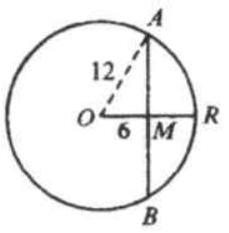
\includegraphics[width=\textwidth]{images/150(1).jpg}

Thus the required chord has length \(12 \sqrt{3}\).\\

\end{document}
